\documentclass[11pt,preprint, authoryear]{elsarticle}

\usepackage{lmodern}
%%%% My spacing
\usepackage{setspace}
\setstretch{1.2}
\DeclareMathSizes{12}{14}{10}{10}

% Wrap around which gives all figures included the [H] command, or places it "here". This can be tedious to code in Rmarkdown.
\usepackage{float}
\let\origfigure\figure
\let\endorigfigure\endfigure
\renewenvironment{figure}[1][2] {
    \expandafter\origfigure\expandafter[H]
} {
    \endorigfigure
}

\let\origtable\table
\let\endorigtable\endtable
\renewenvironment{table}[1][2] {
    \expandafter\origtable\expandafter[H]
} {
    \endorigtable
}


\usepackage{ifxetex,ifluatex}
\usepackage{fixltx2e} % provides \textsubscript
\ifnum 0\ifxetex 1\fi\ifluatex 1\fi=0 % if pdftex
  \usepackage[T1]{fontenc}
  \usepackage[utf8]{inputenc}
\else % if luatex or xelatex
  \ifxetex
    \usepackage{mathspec}
    \usepackage{xltxtra,xunicode}
  \else
    \usepackage{fontspec}
  \fi
  \defaultfontfeatures{Mapping=tex-text,Scale=MatchLowercase}
  \newcommand{\euro}{€}
\fi

\usepackage{amssymb, amsmath, amsthm, amsfonts}

\def\bibsection{\section*{References}} %%% Make "References" appear before bibliography


\usepackage[round]{natbib}

\usepackage{longtable}
\usepackage[margin=2.3cm,bottom=2cm,top=2.5cm, includefoot]{geometry}
\usepackage{fancyhdr}
\usepackage[bottom, hang, flushmargin]{footmisc}
\usepackage{graphicx}
\numberwithin{equation}{section}
\numberwithin{figure}{section}
\numberwithin{table}{section}
\setlength{\parindent}{0cm}
\setlength{\parskip}{1.3ex plus 0.5ex minus 0.3ex}
\usepackage{textcomp}
\renewcommand{\headrulewidth}{0.2pt}
\renewcommand{\footrulewidth}{0.3pt}

\usepackage{array}
\newcolumntype{x}[1]{>{\centering\arraybackslash\hspace{0pt}}p{#1}}

%%%%  Remove the "preprint submitted to" part. Don't worry about this either, it just looks better without it:
\makeatletter
\def\ps@pprintTitle{%
  \let\@oddhead\@empty
  \let\@evenhead\@empty
  \let\@oddfoot\@empty
  \let\@evenfoot\@oddfoot
}
\makeatother

 \def\tightlist{} % This allows for subbullets!

\usepackage{hyperref}
\hypersetup{breaklinks=true,
            bookmarks=true,
            colorlinks=true,
            citecolor=blue,
            urlcolor=blue,
            linkcolor=blue,
            pdfborder={0 0 0}}


% The following packages allow huxtable to work:
\usepackage{siunitx}
\usepackage{multirow}
\usepackage{hhline}
\usepackage{calc}
\usepackage{tabularx}
\usepackage{booktabs}
\usepackage{caption}


\newenvironment{columns}[1][]{}{}

\newenvironment{column}[1]{\begin{minipage}{#1}\ignorespaces}{%
\end{minipage}
\ifhmode\unskip\fi
\aftergroup\useignorespacesandallpars}

\def\useignorespacesandallpars#1\ignorespaces\fi{%
#1\fi\ignorespacesandallpars}

\makeatletter
\def\ignorespacesandallpars{%
  \@ifnextchar\par
    {\expandafter\ignorespacesandallpars\@gobble}%
    {}%
}
\makeatother

\newlength{\cslhangindent}
\setlength{\cslhangindent}{1.5em}
\newenvironment{CSLReferences}%
  {\setlength{\parindent}{0pt}%
  \everypar{\setlength{\hangindent}{\cslhangindent}}\ignorespaces}%
  {\par}


\urlstyle{same}  % don't use monospace font for urls
\setlength{\parindent}{0pt}
\setlength{\parskip}{6pt plus 2pt minus 1pt}
\setlength{\emergencystretch}{3em}  % prevent overfull lines
\setcounter{secnumdepth}{5}

%%% Use protect on footnotes to avoid problems with footnotes in titles
\let\rmarkdownfootnote\footnote%
\def\footnote{\protect\rmarkdownfootnote}
\IfFileExists{upquote.sty}{\usepackage{upquote}}{}

%%% Include extra packages specified by user

%%% Hard setting column skips for reports - this ensures greater consistency and control over the length settings in the document.
%% page layout
%% paragraphs
\setlength{\baselineskip}{12pt plus 0pt minus 0pt}
\setlength{\parskip}{12pt plus 0pt minus 0pt}
\setlength{\parindent}{0pt plus 0pt minus 0pt}
%% floats
\setlength{\floatsep}{12pt plus 0 pt minus 0pt}
\setlength{\textfloatsep}{20pt plus 0pt minus 0pt}
\setlength{\intextsep}{14pt plus 0pt minus 0pt}
\setlength{\dbltextfloatsep}{20pt plus 0pt minus 0pt}
\setlength{\dblfloatsep}{14pt plus 0pt minus 0pt}
%% maths
\setlength{\abovedisplayskip}{12pt plus 0pt minus 0pt}
\setlength{\belowdisplayskip}{12pt plus 0pt minus 0pt}
%% lists
\setlength{\topsep}{10pt plus 0pt minus 0pt}
\setlength{\partopsep}{3pt plus 0pt minus 0pt}
\setlength{\itemsep}{5pt plus 0pt minus 0pt}
\setlength{\labelsep}{8mm plus 0mm minus 0mm}
\setlength{\parsep}{\the\parskip}
\setlength{\listparindent}{\the\parindent}
%% verbatim
\setlength{\fboxsep}{5pt plus 0pt minus 0pt}



\begin{document}



\begin{frontmatter}  %

\title{Evolution of Covid outbreak}

% Set to FALSE if wanting to remove title (for submission)




\author[Add1]{Harriet Laing\footnote{}}
\ead{}





\address[Add1]{Univeristy of Stellenbosch, Cape Town, South Africa}



\vspace{1cm}





\vspace{0.5cm}

\end{frontmatter}



%________________________
% Header and Footers
%%%%%%%%%%%%%%%%%%%%%%%%%%%%%%%%%
\pagestyle{fancy}
\chead{}
\rhead{}
\lfoot{}
\rfoot{\footnotesize Page \thepage}
\lhead{}
%\rfoot{\footnotesize Page \thepage } % "e.g. Page 2"
\cfoot{}

%\setlength\headheight{30pt}
%%%%%%%%%%%%%%%%%%%%%%%%%%%%%%%%%
%________________________

\headsep 35pt % So that header does not go over title




\hypertarget{introduction}{%
\section{\texorpdfstring{Introduction
\label{Introduction}}{Introduction }}\label{introduction}}

This report looks at descriptive statistics to understand the evolution
of Covid-19 in 2020. First, the impact of Covid on Africa countries is
investigated, then the countries with a high prevalence of smoking and
then how quickly different regions increased hospital facilities as
Covid-19 continued throughout the 2020 year.

\hypertarget{data}{%
\section*{Data}\label{data}}
\addcontentsline{toc}{section}{Data}

The data that is used is from Our World in Data and was subsetted to our
period of interest which is 2020.

\hypertarget{investigating-the-misconception-of-the-experience-of-african-countries-with-covid-compared-with-other-regions.}{%
\subsection{Investigating the misconception of the experience of African
countries with Covid compared with other
regions.}\label{investigating-the-misconception-of-the-experience-of-african-countries-with-covid-compared-with-other-regions.}}

\begin{figure}[H]

{\centering \includegraphics{Question1_files/figure-latex/Figure1-1} 

}

\end{figure}

\hypertarget{countries-with-high-prevalence-of-smoking-severity-of-covid}{%
\subsection{Countries with high prevalence of smoking \& severity of
Covid}\label{countries-with-high-prevalence-of-smoking-severity-of-covid}}

According to World Population Review, the countries that have the
highest prevalence of smoking are:

Nauru (52.10\%) Kiribati (52.00\%) Tuvalu (48.70\%) Myanmar (45.50\%)
Chile (44.70\%) Lebanon (42.60\%) Serbia (40.60\%) Bangladesh (39.10\%)
Greece (39.10\%) Bulgaria (38.90\%)

Compare these countries with highest prevalence of smoking to the world
average of new deaths in 2020 from Covid.

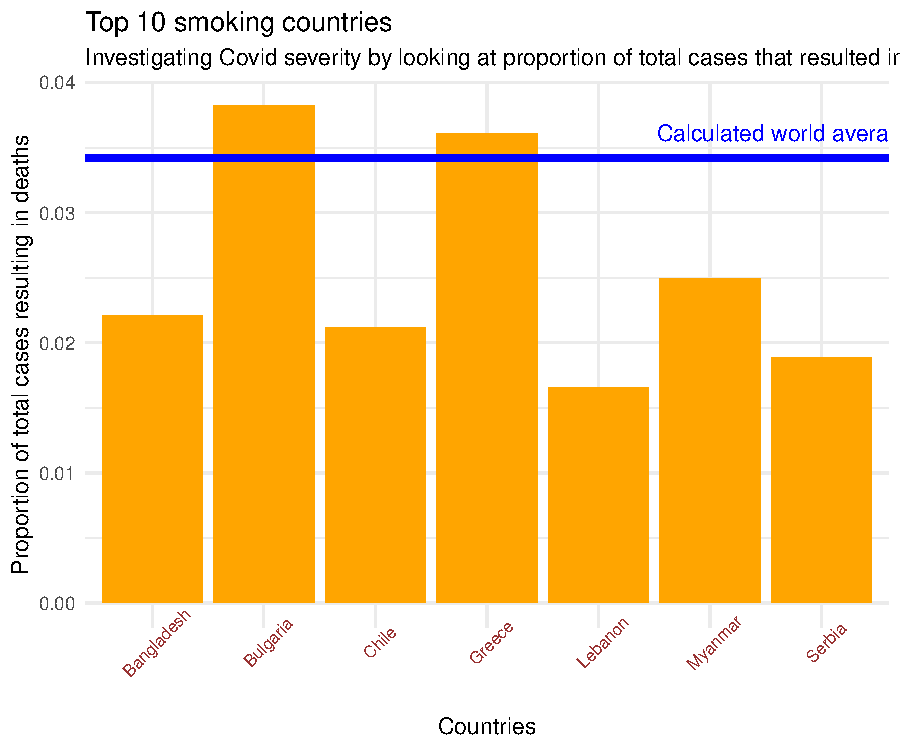
\includegraphics{Question1_files/figure-latex/unnamed-chunk-1-1.pdf}

\hypertarget{how-quickly-did-different-regions-increase-hospitalisation-facilities}{%
\subsection{How quickly did different regions increase hospitalisation
facilities?}\label{how-quickly-did-different-regions-increase-hospitalisation-facilities}}

Did that time series of hospital beds lead or lag on ICU admission
rates? By removing the na values, we subset the data to begin at March
8th.

According to the figures, we can see that generally the rates of
hospitalisations were similar to rates of ICU admission, and
occasionally led on ICU admission. Oceania was excluded because not
enough data, and other regions are missing one of the values due to data
constraints.

\hypertarget{asia}{%
\subsection{Asia}\label{asia}}

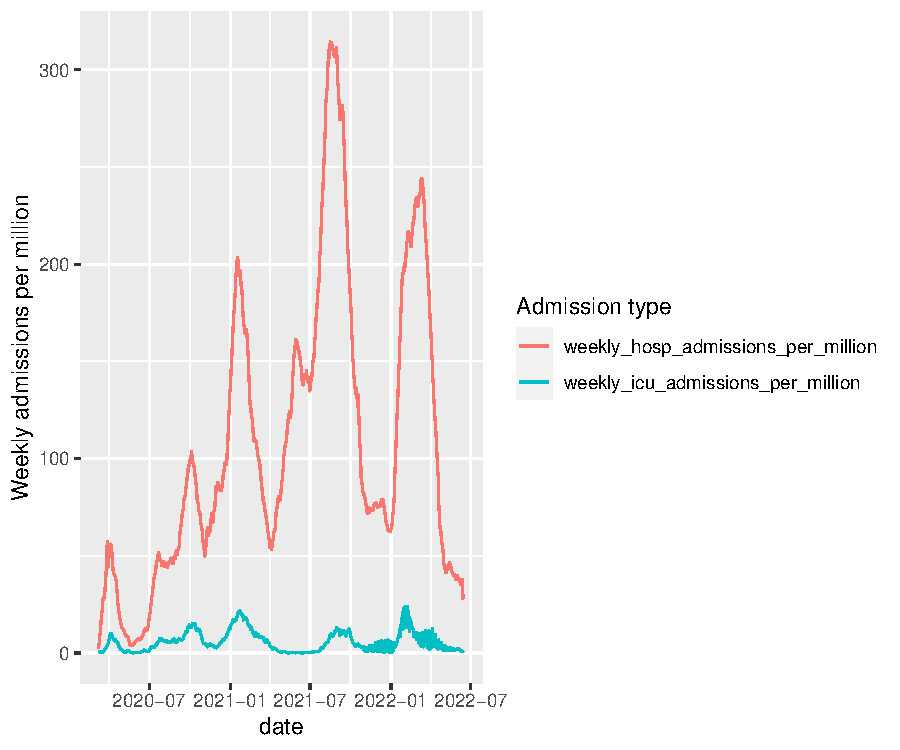
\includegraphics{Question1_files/figure-latex/unnamed-chunk-2-1.pdf}

\hypertarget{africa}{%
\subsection{Africa}\label{africa}}

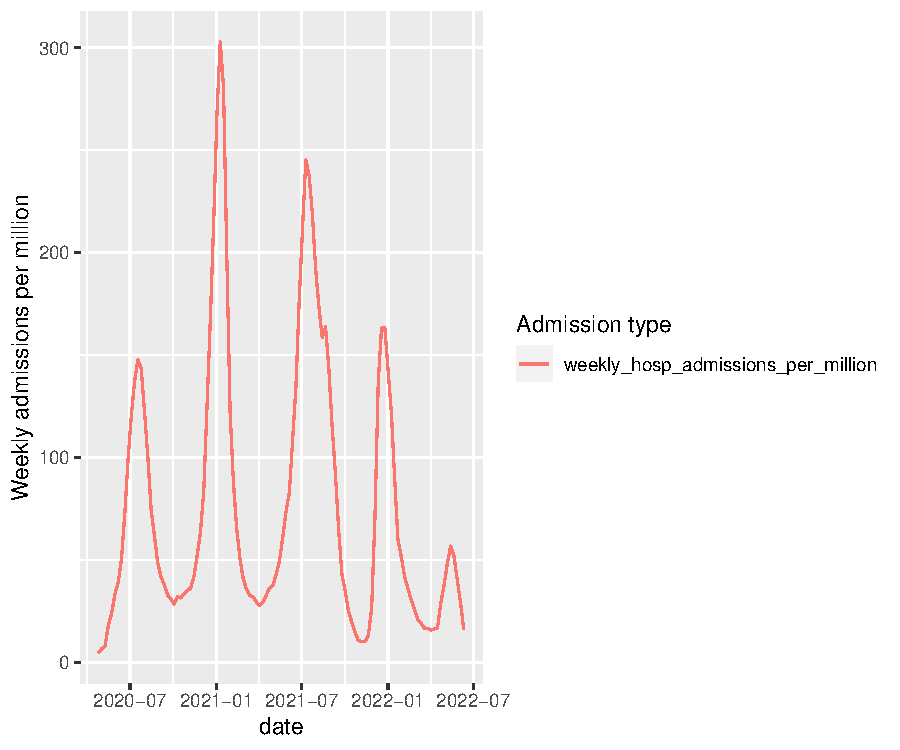
\includegraphics{Question1_files/figure-latex/unnamed-chunk-3-1.pdf}

\hypertarget{europe}{%
\subsection{Europe}\label{europe}}

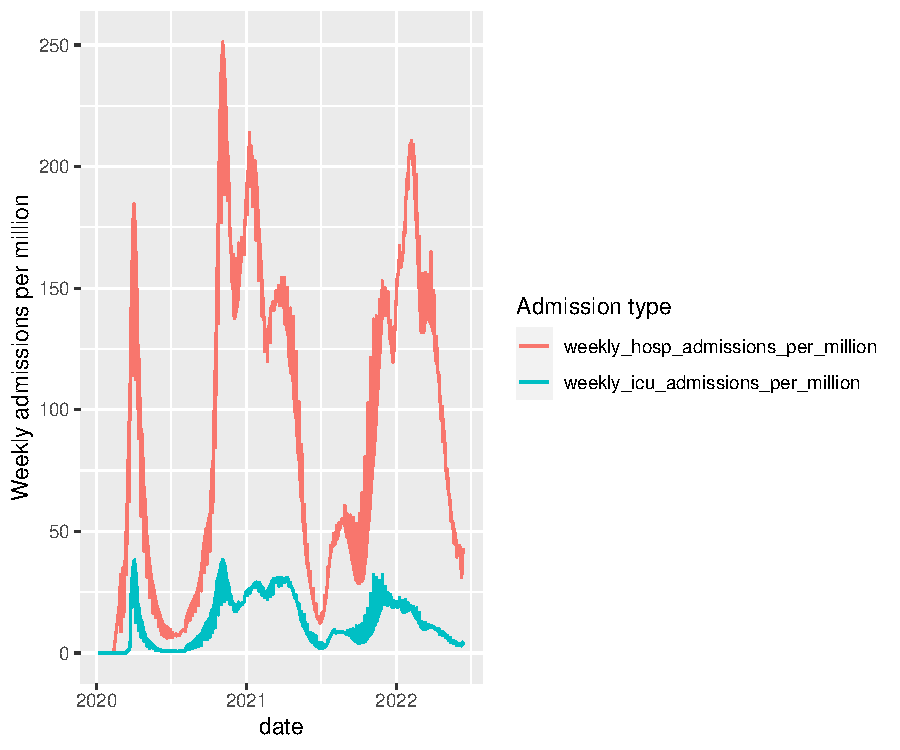
\includegraphics{Question1_files/figure-latex/unnamed-chunk-4-1.pdf}

\hypertarget{north-america}{%
\subsection{North America}\label{north-america}}

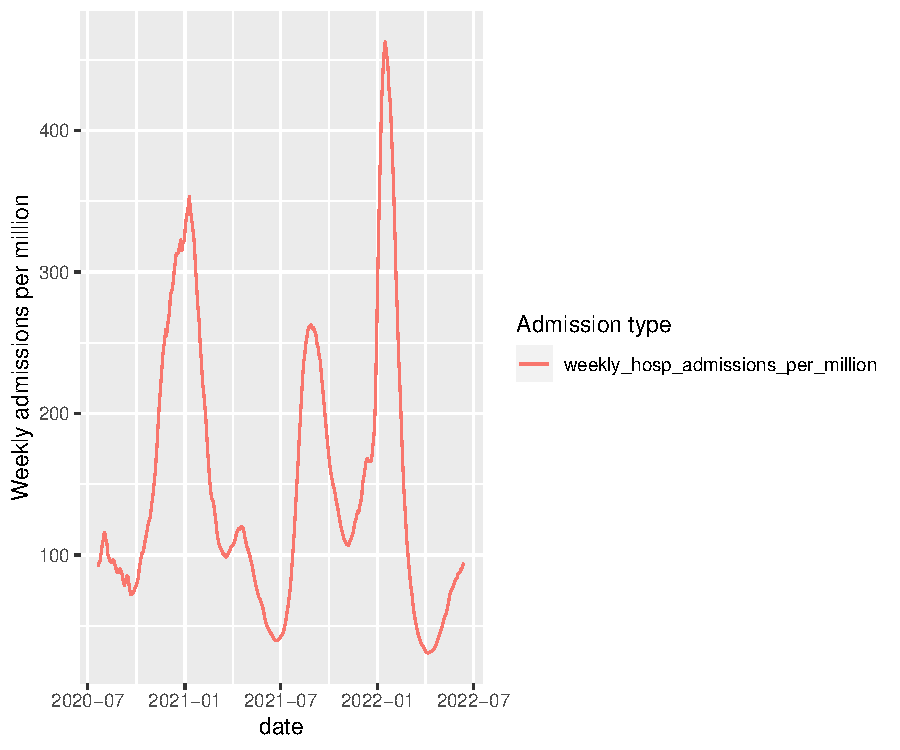
\includegraphics{Question1_files/figure-latex/unnamed-chunk-5-1.pdf}

\hypertarget{south-america}{%
\subsection{South America}\label{south-america}}

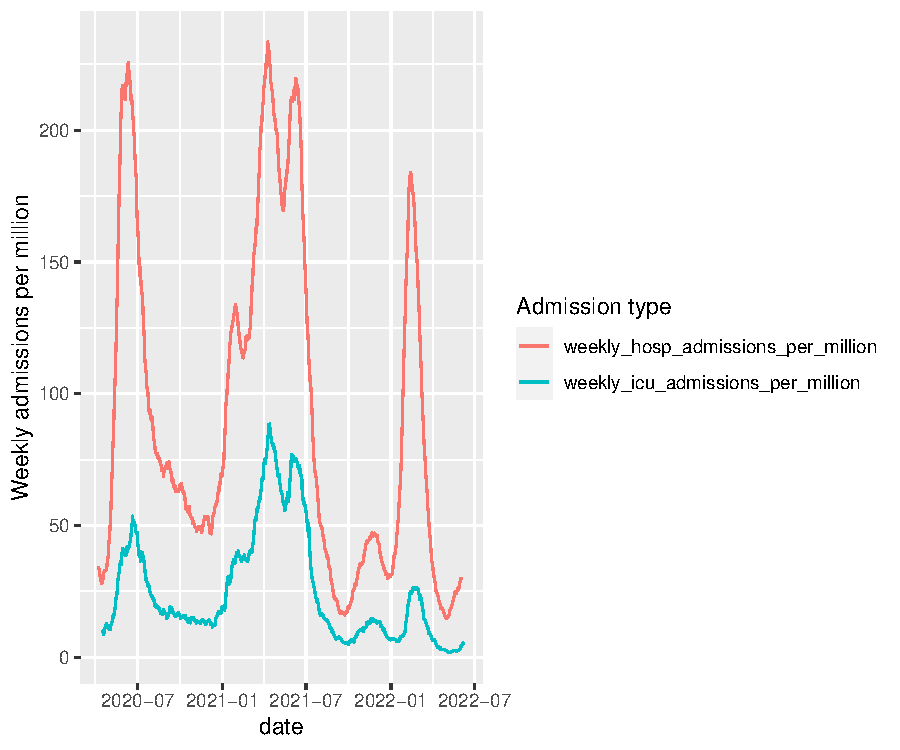
\includegraphics{Question1_files/figure-latex/unnamed-chunk-6-1.pdf}

\bibliography{Tex/ref}





\end{document}
